%%%%%%%%%%%%%%%%%%%%%%%%%%%%%%%%%%%%%%%%%%%%%%
%                insertmeeting
% 1) Title (something creative & funny?)
% 2) Date (MM/DD/YYYY)
% 3) Location (ex. Hagerty High School)
% 4) People/Committees Present 
% 5) Picture 
% 6) Start Time & Stop Time (ex. 12:30AM to 4:30PM)
%%%%%%%%%%%%%%%%%%%%%%%%%%%%%%%%%%%%%%%%%%%%%%
\insertmeeting 
  {Car Drivetrain} 
  {10/14/21}
  {Hagerty High School}
  {Annika, Anouska, Clayton, Falon, Jensen, Nathan, Ritam, Rose, Samantha}
  {Images/RobotPics/robot.jpg}
  {2:30 - 4:30}
  
\hhscommittee{General}
\noindent\hfil\rule{\textwidth}{.4pt}\hfil
\subsubsection*{Goals}
\begin{itemize}
    \item Test drive car drivetrain  

\end{itemize} 

\noindent\hfil\rule{\textwidth}{.4pt}\hfil

\subsubsection*{Accomplishments}
Today we hit a major milestone with our car drivetrain as we drove it around the field for the first time. We had a lot of fun driving it, as it controls very differently to any other robot we’ve ever seen (Figure \ref{fig:pic1}). As the name suggests, it drives more like a car because of its front wheel turning. Despite being very different, controlling the robot started to feel pretty natural as we practiced making cycles. Even without any arm or other mechanism attached, we found that we could drive as fast as the tank drivetrain, and with a little practice, we could be moving extremely quickly. We all were in agreement that this drivetrain has a lot more potential for speed than the tank drive does. With all of this in mind, we decided to continue working with this 3- wheeled car drivetrain, giving hardware the task of designing a 3d printed version.

\begin{figure}[htp]
\centering
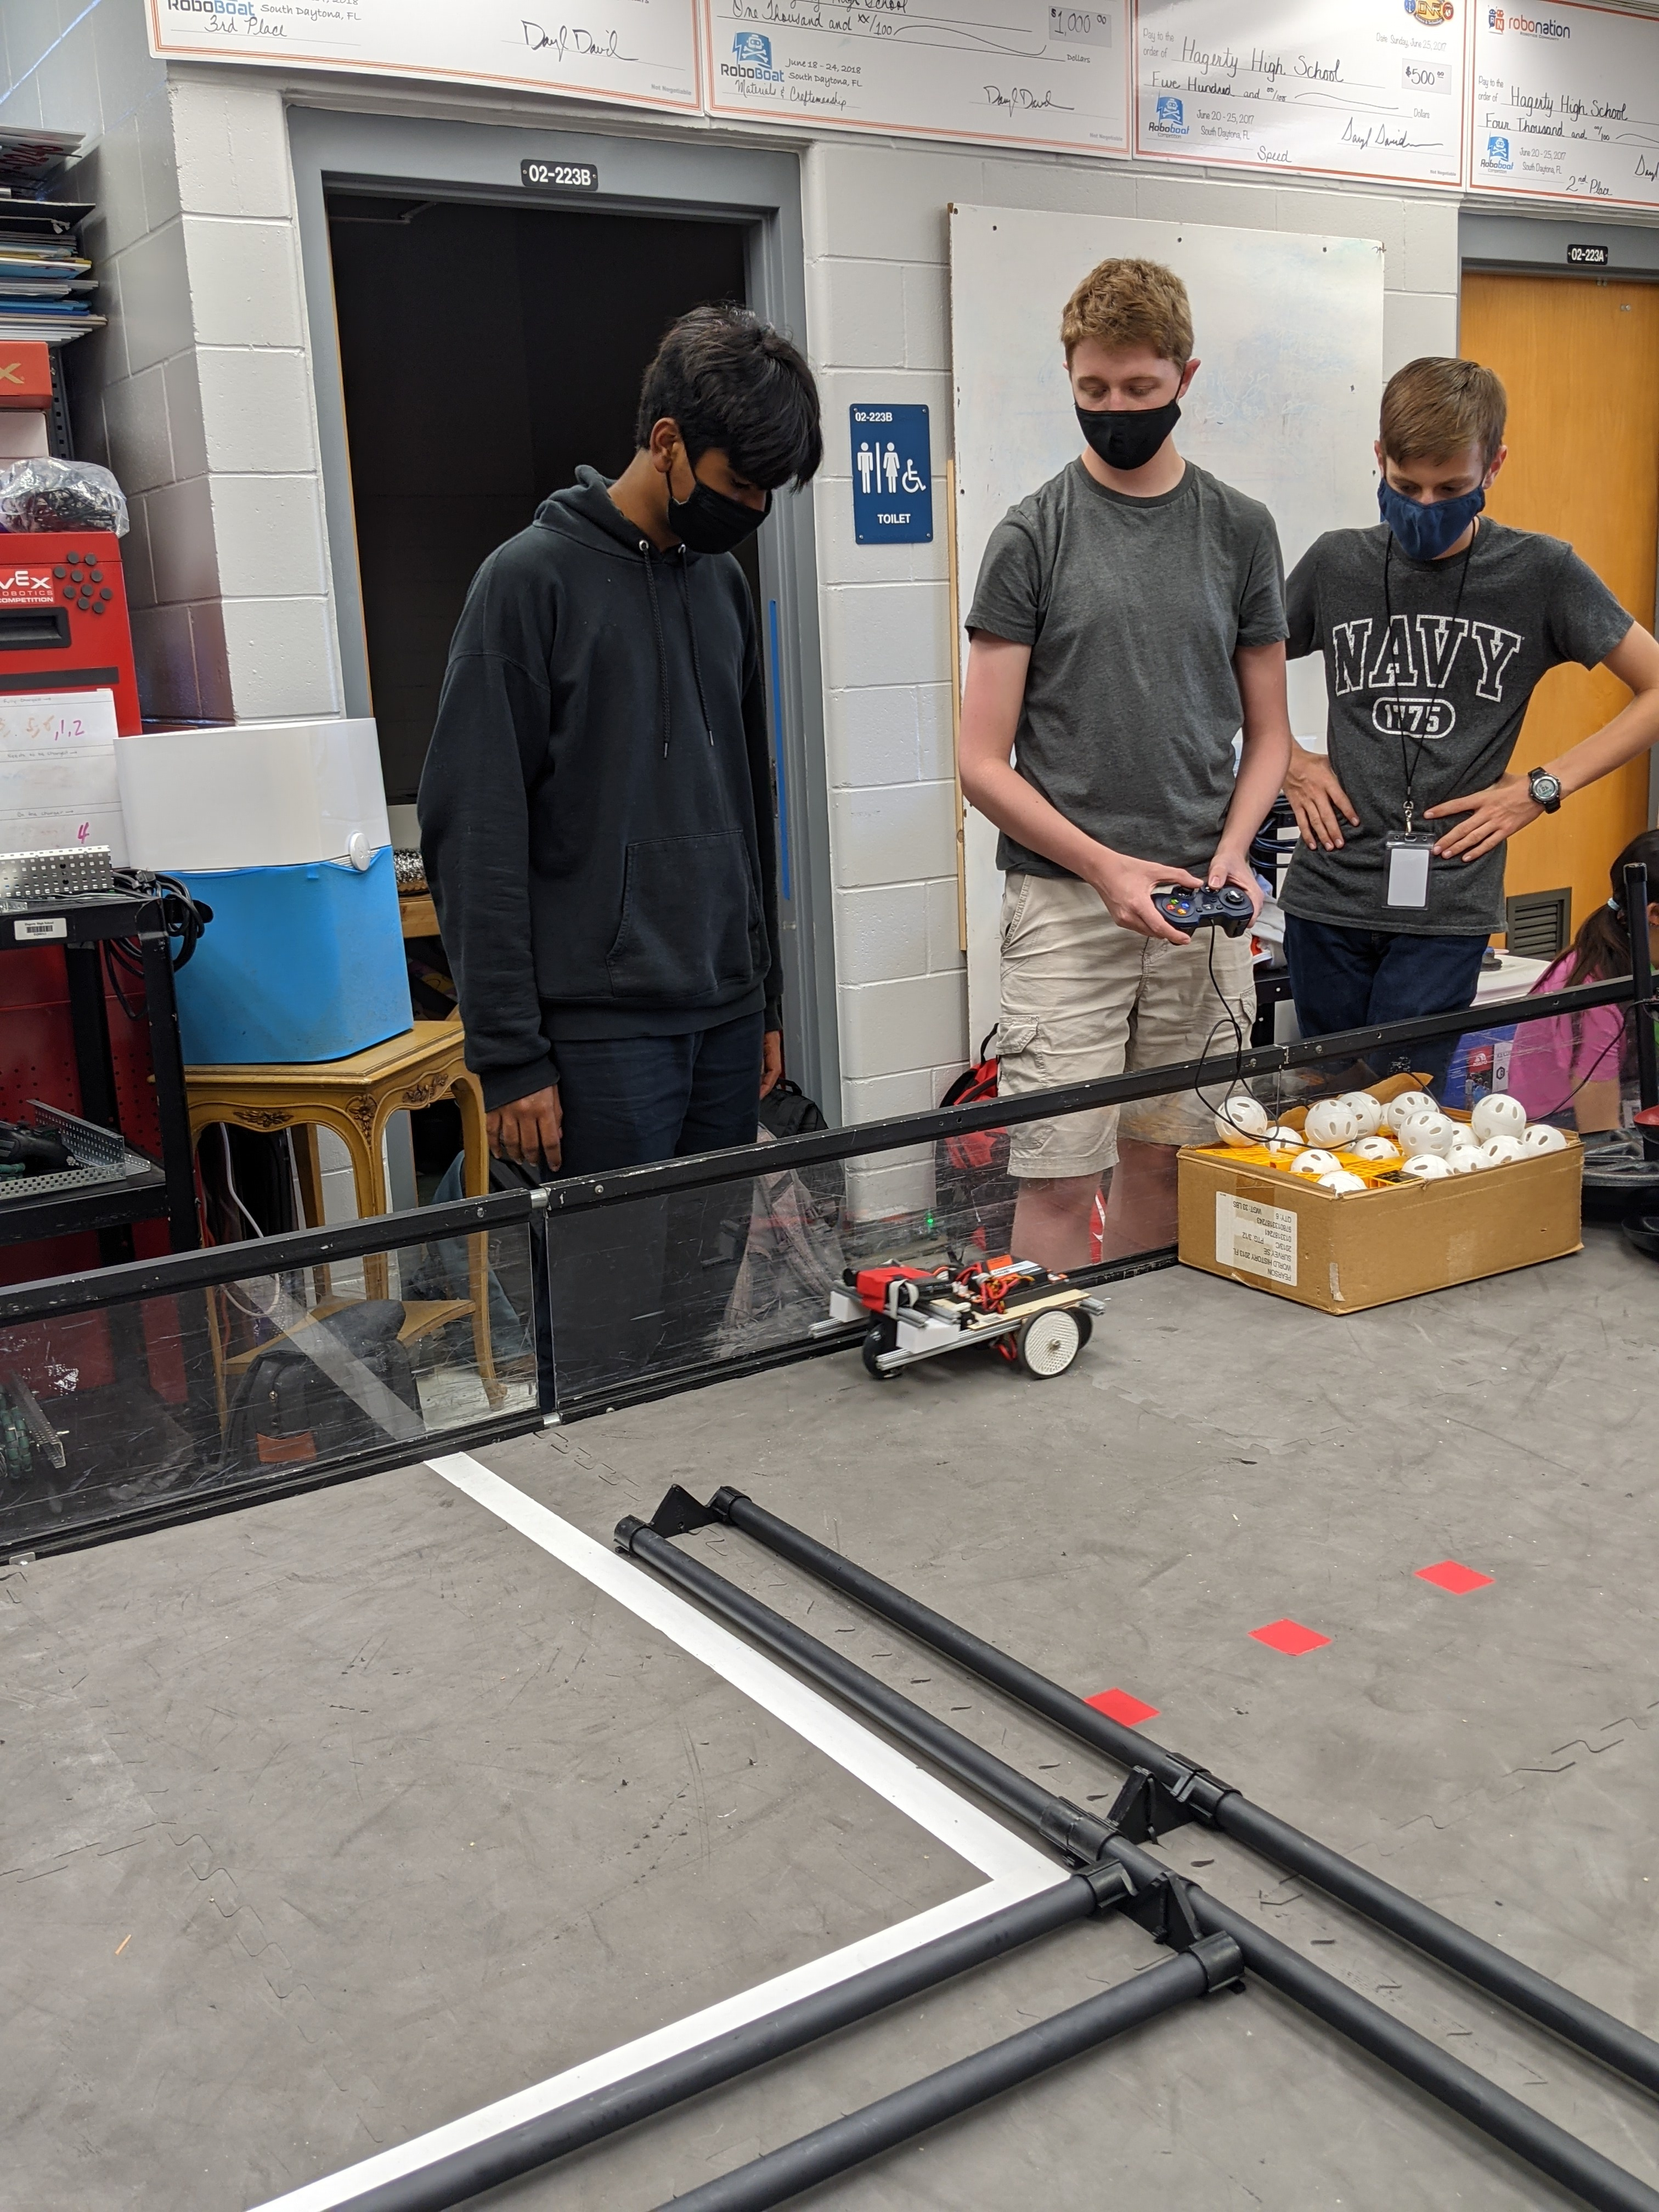
\includegraphics[width=0.95\textwidth, angle=0]{Meetings/October/10-14-21/10-14-21_Team_Figure1 - Nathan Forrer.jpg}
\caption{Ritam and Nathan driving the new drivetrain.}
\label{fig:pic1}
\end{figure}

\hhscommittee{Hardware}
\noindent\hfil\rule{\textwidth}{.4pt}\hfil
\subsubsection*{Goals}
\begin{itemize}
    \item Design a 3d printable drivetrain

\end{itemize} 

\noindent\hfil\rule{\textwidth}{.4pt}\hfil

\subsubsection*{Accomplishments}
Today, we started on one of our most daunting tasks yet: designing a 3d printable drivetrain. One of the main challenges of creating this drivetrain is that we have to make it very strong so that it doesn't break when we hit another robot, but we also must keep it light. Seeing the success of the 3 wheeled car drivetrain prototype, we decided that it would be the design we would create. We started making the drivetrain in CAD, designing it around a large rectangular top plate that we can attach electronics and other mechanisms to. Much like with our prototype design, we had to stagger the motors to keep the robot small, but this time we moved the motors towards the front of the robot and plan on connecting them using pulleys (Figure \ref{fig:pic2}). After creating all of the basics, we added strength to the design, using ribs, chamfers and fillets to make the structure more rigid without adding too much weight (Figure \ref{fig:pic3}). Using structures like this allowed us to use 1/8 inch sides for most of the robot, when we normally use 1/4 inch. By being smart about where to add structure, such as around the motors and at other key points, we were able to find what we think is a good balance between strength and weight.

\begin{figure}[ht]
\centering
\begin{minipage}[b]{.48\textwidth}
  \centering
  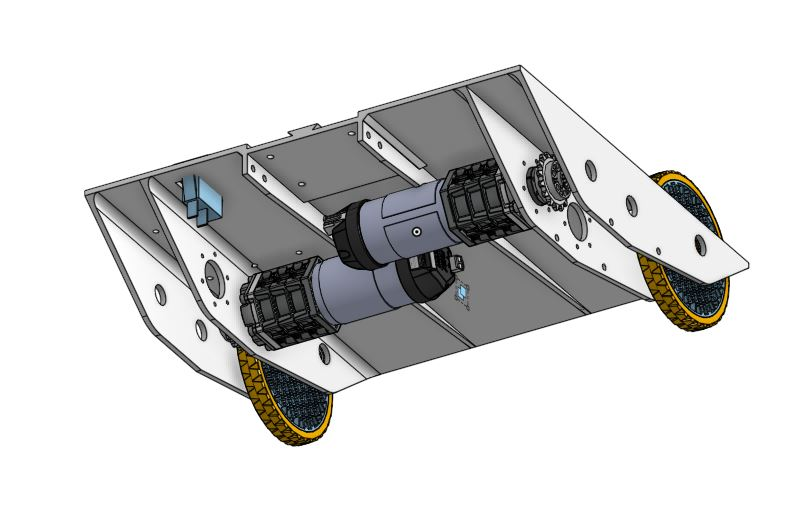
\includegraphics[width=0.95\textwidth]{Meetings/October/10-14-21/10-14-21_CAD_Figure1.JPG}
  \caption{Current CAD of our drivetrain.}
  \label{fig:pic2}
\end{minipage}%
\hfill%
\begin{minipage}[b]{.48\textwidth}
  \centering
  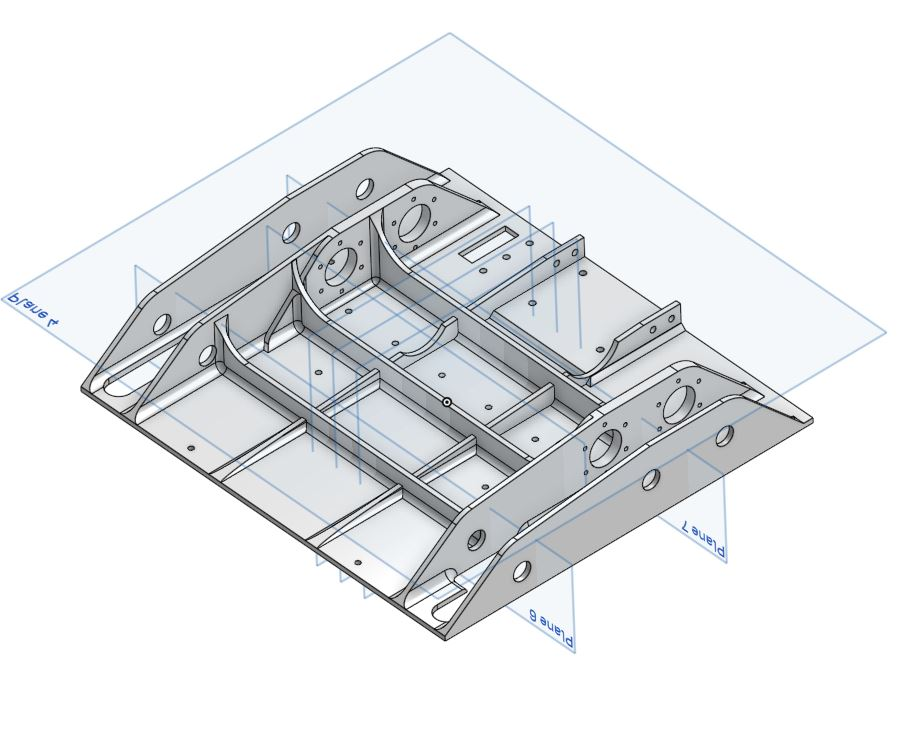
\includegraphics[width=0.95\textwidth]{Meetings/October/10-14-21/10-14-21_CAD_Figure2.JPG}
  \caption{Our drivetrain's 3D printed base.}
  \label{fig:pic3}
\end{minipage}
\end{figure}

\begin{figure}[htp]
\centering
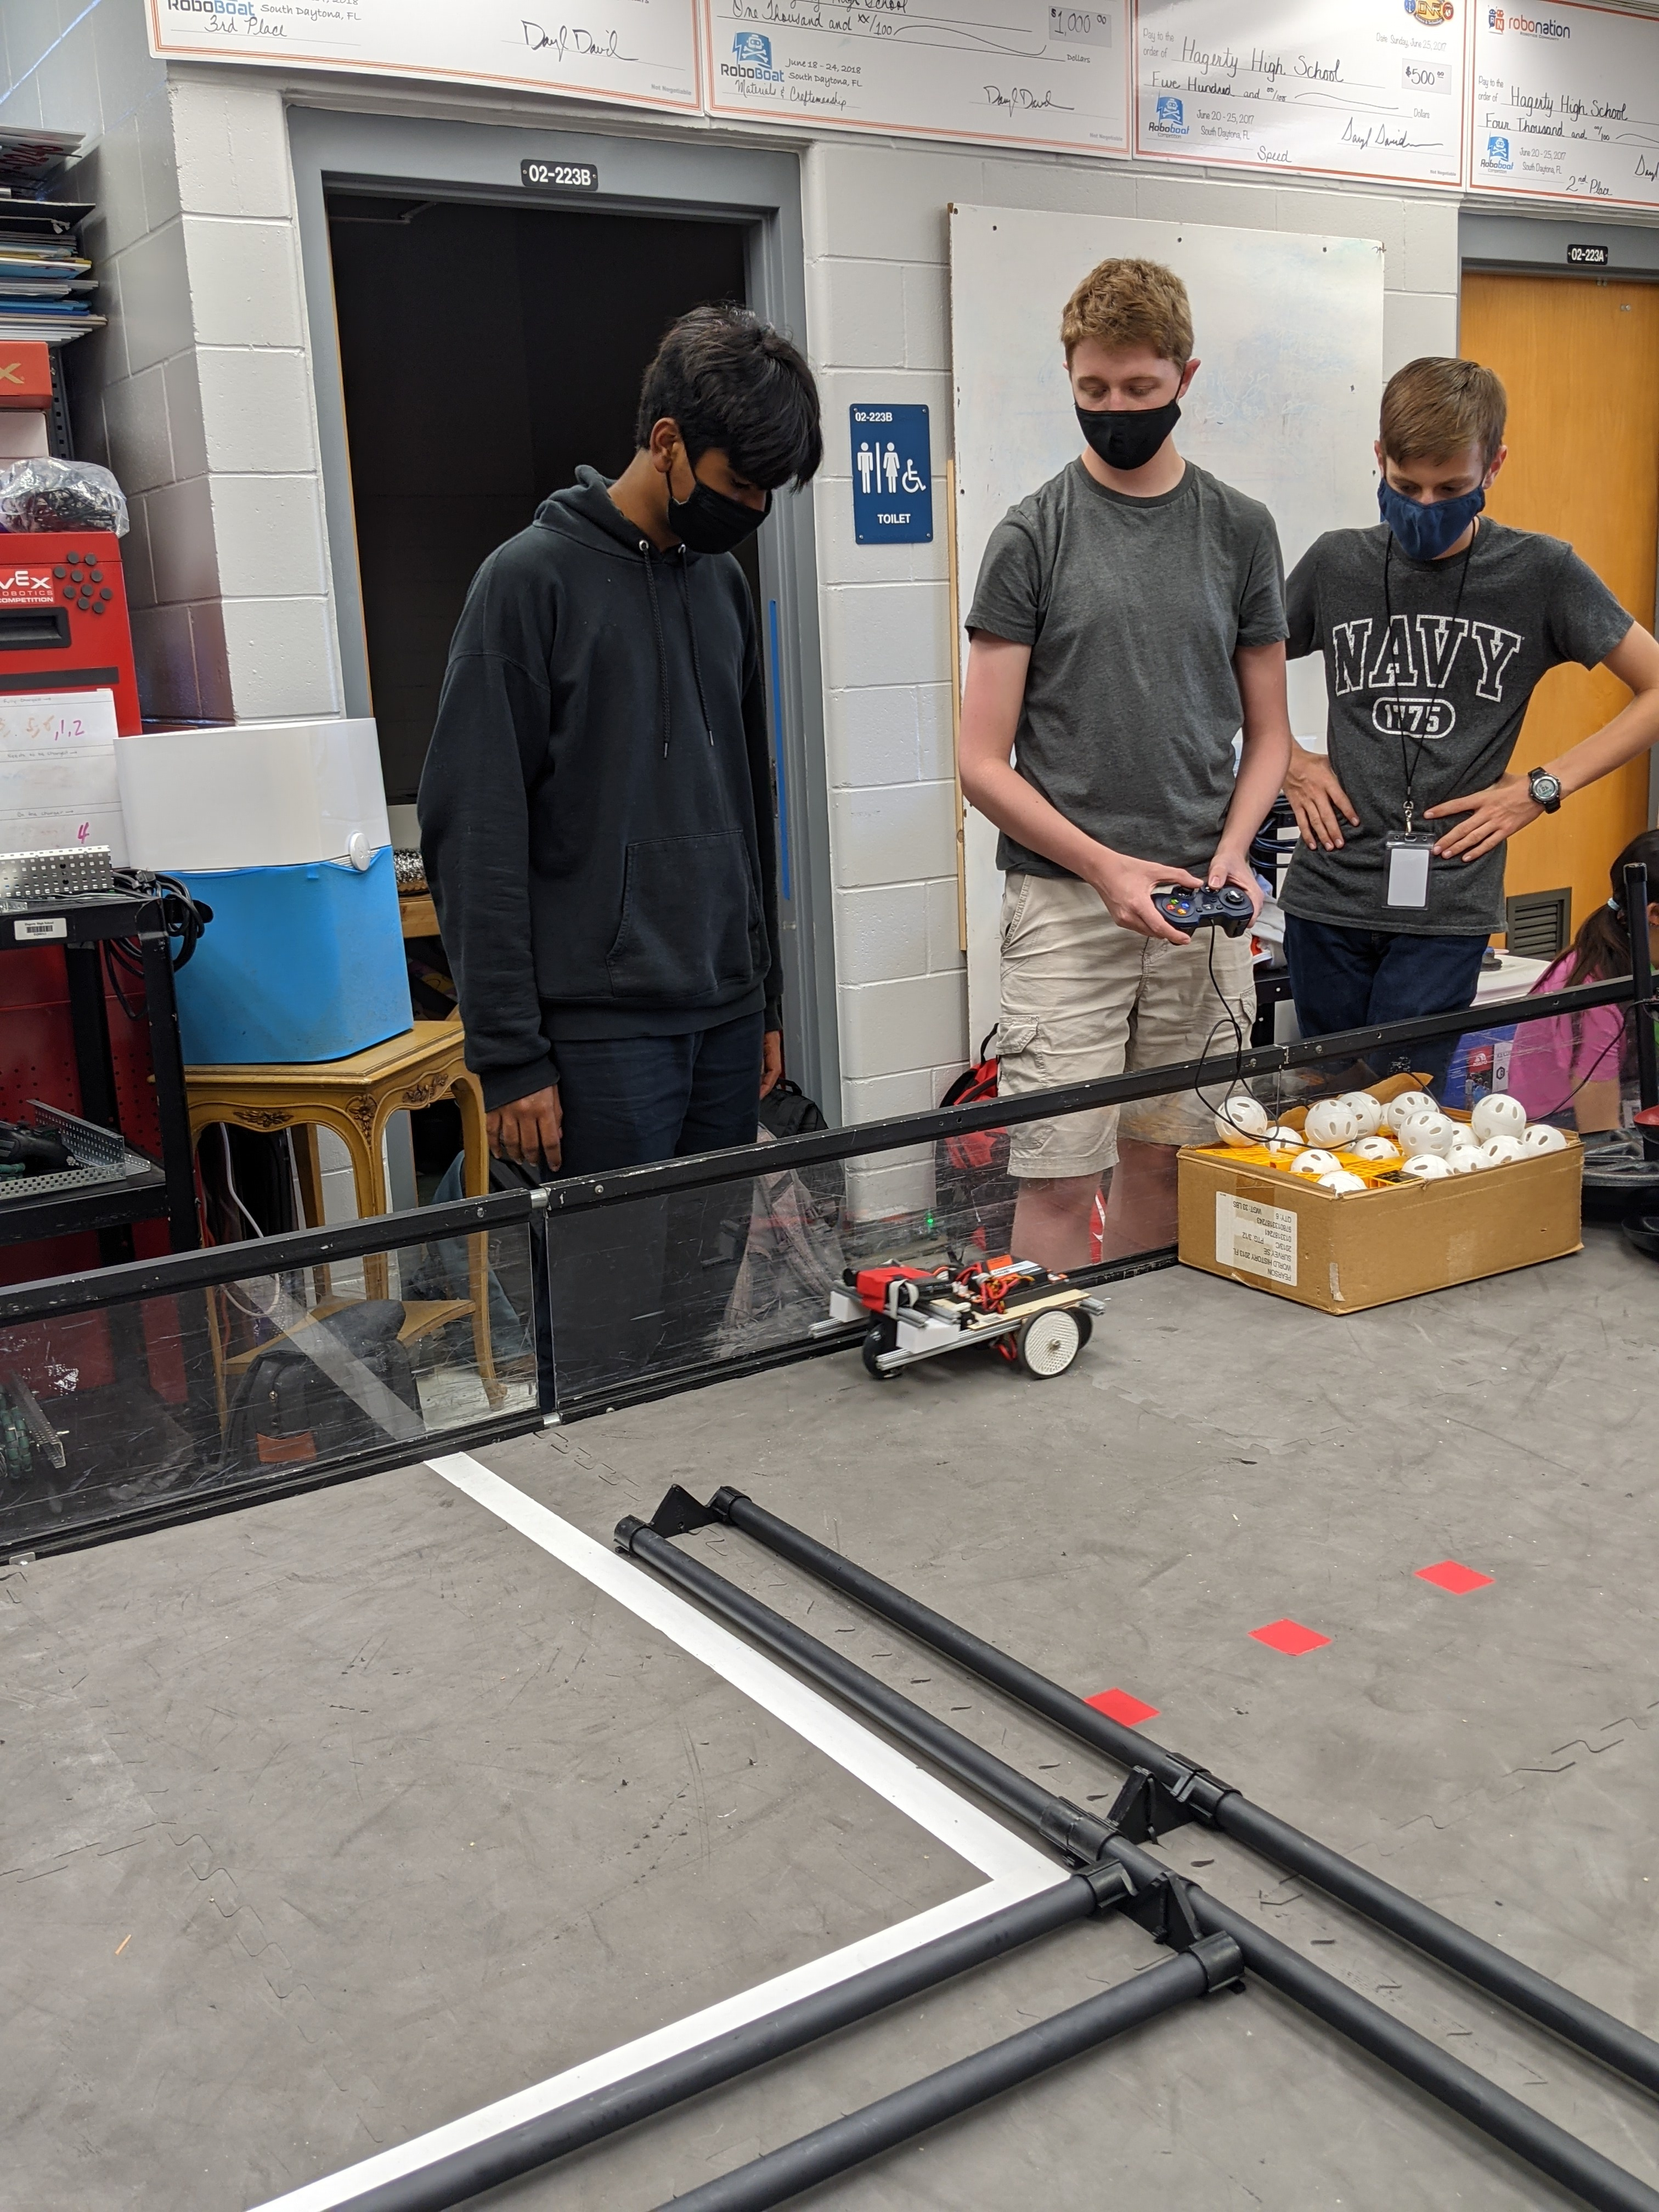
\includegraphics[width=0.95\textwidth, angle=0]{Meetings/October/10-14-21/10-14-21_Team_Figure1 - Nathan Forrer.jpg}
\caption{Ritam and Nathan driving the new drivetrain.}
\label{fig:pic1}
\end{figure}

\hhscommittee{Hardware}
\noindent\hfil\rule{\textwidth}{.4pt}\hfil
\subsubsection*{Goals}
\begin{itemize}
    \item Design a 3d printable drivetrain

\end{itemize} 

\noindent\hfil\rule{\textwidth}{.4pt}\hfil

\subsubsection*{Accomplishments}
Today, we started on one of our most daunting tasks yet: designing a 3d printable drivetrain. One of the main challenges of creating this drivetrain is that we have to make it very strong so that it doesn't break when we hit another robot, but we also must keep it light. Seeing the success of the 3 wheeled car drivetrain prototype, we decided that it would be the design we would create. We started making the drivetrain in CAD, designing it around a large rectangular top plate that we can attach electronics and other mechanisms to. Much like with our prototype design, we had to stagger the motors to keep the robot small, but this time we moved the motors towards the front of the robot and plan on connecting them using pulleys (Figure \ref{fig:pic2}). After creating all of the basics, we added strength to the design, using ribs, chamfers and fillets to make the structure more rigid without adding too much weight (Figure \ref{fig:pic3}). Using structures like this allowed us to use 1/8 inch sides for most of the robot, when we normally use 1/4 inch. By being smart about where to add structure, such as around the motors and at other key points, we were able to find what we think is a good balance between strength and weight.

\begin{figure}[ht]
\centering
\begin{minipage}[b]{.48\textwidth}
  \centering
  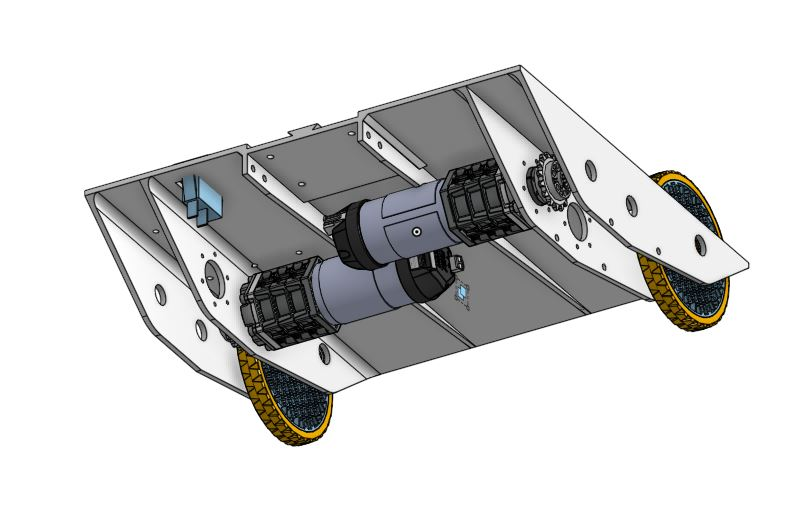
\includegraphics[width=0.95\textwidth]{Meetings/October/10-14-21/10-14-21_CAD_Figure1.JPG}
  \caption{Current CAD of our drivetrain.}
  \label{fig:pic2}
\end{minipage}%
\hfill%
\begin{minipage}[b]{.48\textwidth}
  \centering
  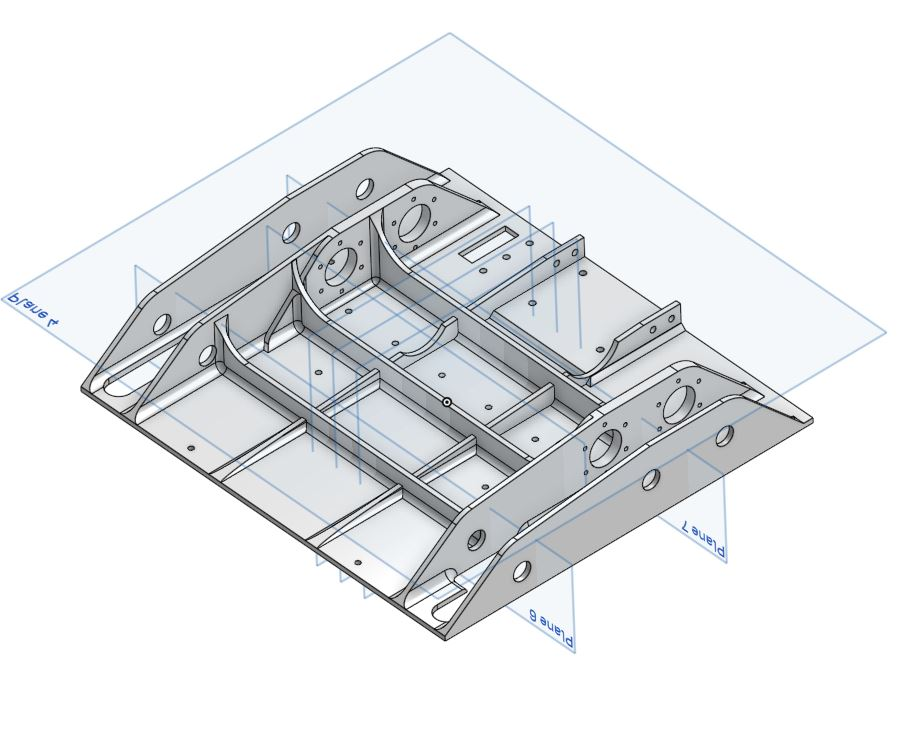
\includegraphics[width=0.95\textwidth]{Meetings/October/10-14-21/10-14-21_CAD_Figure2.JPG}
  \caption{Our drivetrain's 3D printed base.}
  \label{fig:pic3}
\end{minipage}
\end{figure}

\hhscommittee{Outreach}
\noindent\hfil\rule{\textwidth}{.4pt}\hfil
\subsubsection*{Goals}
\begin{itemize}
    \item Installed programming software and prepared for programming for fll
    \item Divided students into 3 teams
 
\end{itemize} 

\noindent\hfil\rule{\textwidth}{.4pt}\hfil

\subsubsection*{Accomplishments}
As our twice a week FLL meetings continue, we are finally moving very close to getting started with the season. At our meeting next Friday, we will finally divide the students up into their competition teams, where they will build their base robots, program their missions, and create their innovation projects. Although we are still a week away from putting them into teams, we started thinking of how we can group them. We decided that the best way for them to get the best out of the program would be to divide them up both by skill and age so that they are all working with teammates with a similar general skill set. To get our thoughts on paper, we created a spreadsheet and put participants in 3 teams tentatively named the minimancers (the most experienced team), the blue team (the medium experience team), and the red team (the beginner team)(Figure \ref{fig:pic4}). For this week though, we will test how these groups work by giving them core values activities to do with their future team members.
Additionally, we started downloading the ev3 programming software onto some of the robotics laptops so that we can start teaching the fll members the basics of programming. Because programming is one of the more complicated and important skills, we plan on doing the basic, more easy programming as a large group, then showing the more experienced teams advanced programming once they’ve been put into their competition teams.

\begin{figure}[htp]
\centering
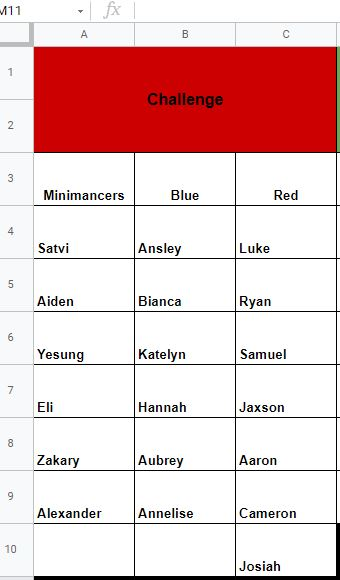
\includegraphics[width=0.95\textwidth, angle=0]{Meetings/October/10-14-21/10-14-21_Outreach_Figure1 - Nathan Forrer.JPG}
\caption{The new FLL teams.}
\label{fig:pic4}
\end{figure}

\whatsnext{
\begin{itemize}
    \item Design 3d printed drivetrain
    \item Add front wheel structure
    \item Start printing the robot
    \item Ensure teams work well together
    \item Get started with the competition!


\end{itemize} 
}

